\section{Bibliothèques de calcul}
(Retour sur l'exemple de la page \pageref{solve})\label{lu}

\`A quelle vitesse peut calculer une machine contemporaine? Résoudre
un système linéaire de n équations à n inconnues est un bon test.

Regardons le programme python suivant (vous pouvez sauter directement à
la ligne \ding{42}):

\begin{verbatim}
     1	import numpy as np
     2	from scipy.linalg import lu_factor,lu_solve
     3	import time
     4	n=5000
     5	A=np.random.rand(n,n)
     6	B=np.random.rand(n)
     7	#
     8	c1=time.time()
     9	lu, piv = lu_factor(A)
    10	X= lu_solve((lu,piv),B)
    11	c2=time.time()
    12	#
    13	n3= 2.*n**3/3.
    14	t=c2-c1
    15	gflops=n3/t/10**9
    16	print("Gigaflops",gflops)    
\end{verbatim}
Passons sur les lignes 1 à 3; aux lignes 4,5 et 6 on fabrique un tableau
au hasard de taille $5000$ par $5000$, et un second membre B de taille
$5000$. Les deux tableaux définissent le système d'équations.
La résolution du système de  $5000$ équations est effectuée aux
lignes 9 et 10. Comme ces lignes  sont entourées de deux mesures de
``l'heure'', la différence (ligne 14) donne le temps calcul t en
secondes.

\ding{42} Le jeu commence ici:
\begin{enumerate}
\item On peut montrer que la résolution (par la méthode de Gauss, qui
  est à peu près celle qu'on apprend au collège) \og coûte\fg{}
  $\frac{2}{3} n^3$ opérations (additions et multiplications) pour un
  système de $n$ équations, donc ici $\frac{2}{3} \times 5000^3$
  opérations soit
  $\frac{2}{3} \times 125 \times 10^9$ opérations (environ $83,33...$
  milliards d'opérations). 
\item Sur ma machine (Intel i5, 3,5 Ghz, 4 c{\oe}urs), le temps calcul est
  de 0.779 secondes.
\end{enumerate}

Donc, ma machine est capable d'effectuer $\frac{2}{3} \times 125 \times
  10^9/ 0.779$ opérations par seconde, soit environ \textbf{106
    milliards d'opérations par seconde!} (on dit: 106,9 gigaflops).

  Diable! Comment est-ce
  possible?

\begin{itemize}
  \item La machine tourne à $3.5$ Gigahertz, ce qui permet à
    \emph{chaque c{\oe}ur} d'effectuer $3,5$ milliards d'opérations par
    seconde.
  \item Mais, ma machine a 4 c{\oe}urs, et le programme est
    ``multithreadé'' (parallélisé sur les 4 c{\oe}urs), donc on peut
    atteindre $4 \times 
    3.5\times 10^9  = 14 $ Gigaflops. Mais ça ne suffit pas à expliquer les 106,9
    gigaflops observés.
  \item La réponse vient des instructions ``avx'' des processeurs
    Intel.
    Supposons qu'on ait 4 ``vecteurs'' w,x,y et z de taille
    4\footnote{C'est l'AVX 256 ($256 = 4 \times 64$). Les derniers
      processeurs ont un AVX 512 (vecteurs de taille 8).} (voir la
    figure \ref{avx});
    alors, les instructions avx permettent de calculer $w= x \times y + z$ en
    \emph{un seul tour d'horloge}\footnote{Pour être plus précis:
      
      \ttt{pour i= 1 à 4:}$w_i = x_i \times y_i + z_i$

      est effectué en  parallèle.}, soit 8 opérations (4 additions et 4
    multiplications) par tour d'horloge. Chaque c{\oe}ur, quand il
    rencontre ce genre d'opération peut donc atteindre la vitesse de
    $3,5 \times 8 = 28$ gigaflops (milliards d'opérations par seconde).
    Donc la vitesse maximale de ma machine (il y a 4 c{\oe}urs) est de
    $4 \times 28 = 112$ gigaflops.
\end{itemize}

Comment est effectué le calcul dans mon programme? En fait, les lignes
11 et 12 passent la main à la bibliothèque \ttt{lapack} (libre et
optimisée pour chaque type de machine). Écrire des programmes qui
permettent d'approcher d'aussi près les
performances théoriques de la machine (106 pour 112) est difficile
(c'est quasiment 
un métier en soi): \textbf{il faut utiliser des bibliothèques!}\medskip


\begin{figure}
  \begin{center}
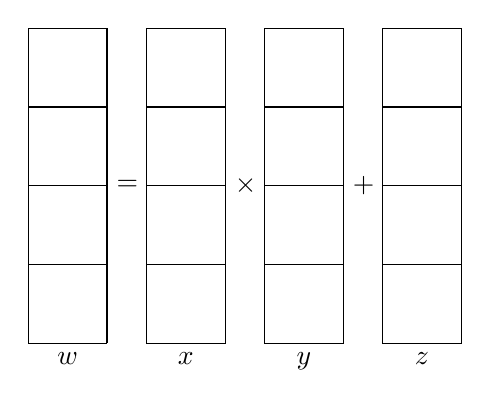
\begin{tikzpicture}
  \draw (0,0) -- (0,4);
  \draw (0,4) -- (1,4);
  \draw (1,4) -- (1,0);
  \draw (1,0) -- (0,0);
  \draw (0,1) -- (1,1);
  \draw (0,2) -- (1,2);
  \draw (0,3) -- (1,3);
  \draw (0.5,0) node [below] {$w$};
  \draw (1,2) node [right] {$=$};
  (1.5,0) rectangle (1.5,4);
  \draw (1.5,0) rectangle (2.5,4);
  \draw (1.5,1) -- (2.5,1);
  \draw (1.5,2) -- (2.5,2);
  \draw (1.5,3) -- (2.5,3);
  \draw (2,0) node [below] {$x$};
  \draw (2.5,2) node [right] {$\times$};

  \draw (3,0) rectangle (4,4);
  \draw (3,1) -- (4,1);
  \draw (3,2) -- (4,2);
  \draw (3,3) -- (4,3);
  \draw (3.5,0) node [below] {$y$};
  \draw (4,2) node [right] {$+$};

   \draw (4.5,0) rectangle (5.5,4);
   \draw (4.5,1) -- (5.5,1);
   \draw (4.5,2) -- (5.5,2);
   \draw (4.5,3) -- (5.5,3);
   \draw (5,0) node [below] {$z$};
\end{tikzpicture}
\end{center}
\caption{AVX (256)}
\label{avx}
\end{figure}
 Remarque finale: il y a là deux types de parallélisme:
  \begin{enumerate}
    \item Les 4 c{\oe}urs font (peuvent faire) des calculs différents
    sur des données différentes: on parle de parallélisme
    \textsf{MIMD} (Multiple Instructions Multiple Data).
    \item Les instructions ``avx'': ont fait en parallèle le même
    calcul sur des données différentes ($w_i = x_i\times y_i + z_i$). On
    parle de parallélisme \textsf{SIMD} (Single Instruction Multiple
    Data). C'est ce que font les GPUs\footnote{Processeurs
      graphiques.}  qui ont de très nombreux c{\oe}urs de calcul (7000
    environ pour les plus puissantes), mais les c{\oe}urs font tous la même
    chose au même moment (idéal 
    pour aditionner deux tableaux, terme à terme): si vous avez 7000
    c{\oe}urs cadencés seulement à une vitesse de 1 Ghz (les GPUs ont
      des vitesses d'horloge relativement faibles), vous atteindrez
      donc la vitesses de $7000 \times 10^9$ opérations par seconde,
      soit 7 téraflops ($ 7 000$ milliards d'opérations par seconde).

      Les derniers processeurs Intel ont, pour chaque c{\oe}ur,
      \emph{deux} unités avx de 512 bits (au lieu de 256) qui
      permettent de calculer
      sur des vecteurs de taille 8 au lieu de 4. La vitesse maximale
      \emph{théorique} de chaque c{\oe}ur est donc $2 \times 16 = 32$
      fois la fréquence d'horloge.
  \end{enumerate}
